% =============================================================================================
% Appendix
% =============================================================================================
\section{Exploratory data analysis (supplementary figures)}
\label{app:eda}
\setcounter{figure}{0}
\renewcommand{\thefigure}{S\arabic{figure}}

\begin{figure}[!htbp]
  \centering
  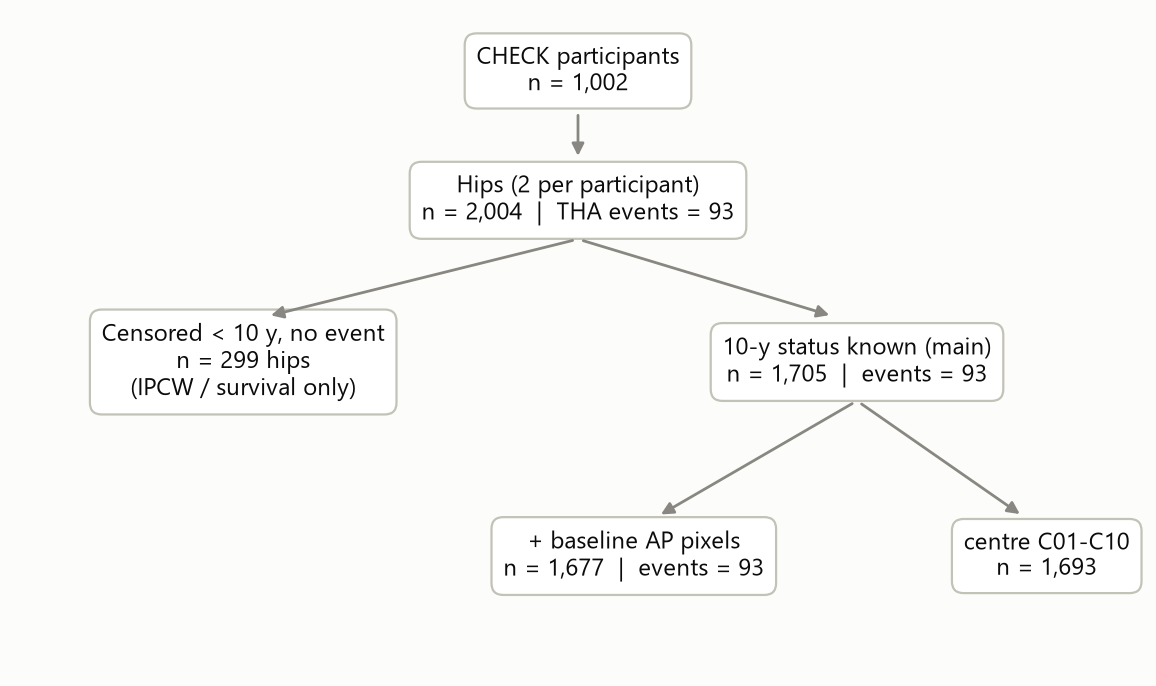
\includegraphics[width=0.78\linewidth]{figS1_flow.png}
  \caption{\textbf{Cohort flow.} 1,002 participants contribute 2,004 hips and 93 THAs. The 299 hips censored before
  year 10 without an event are excluded from the binary analysis and enter only the discrete-time head. Of the 1,705
  hips with known status, 1,677 have baseline AP pixels (every THA hip), and 1,693 belong to a recovered centre.}
  \label{fig:s-flow}
\end{figure}

\begin{figure}[!htbp]
  \centering
  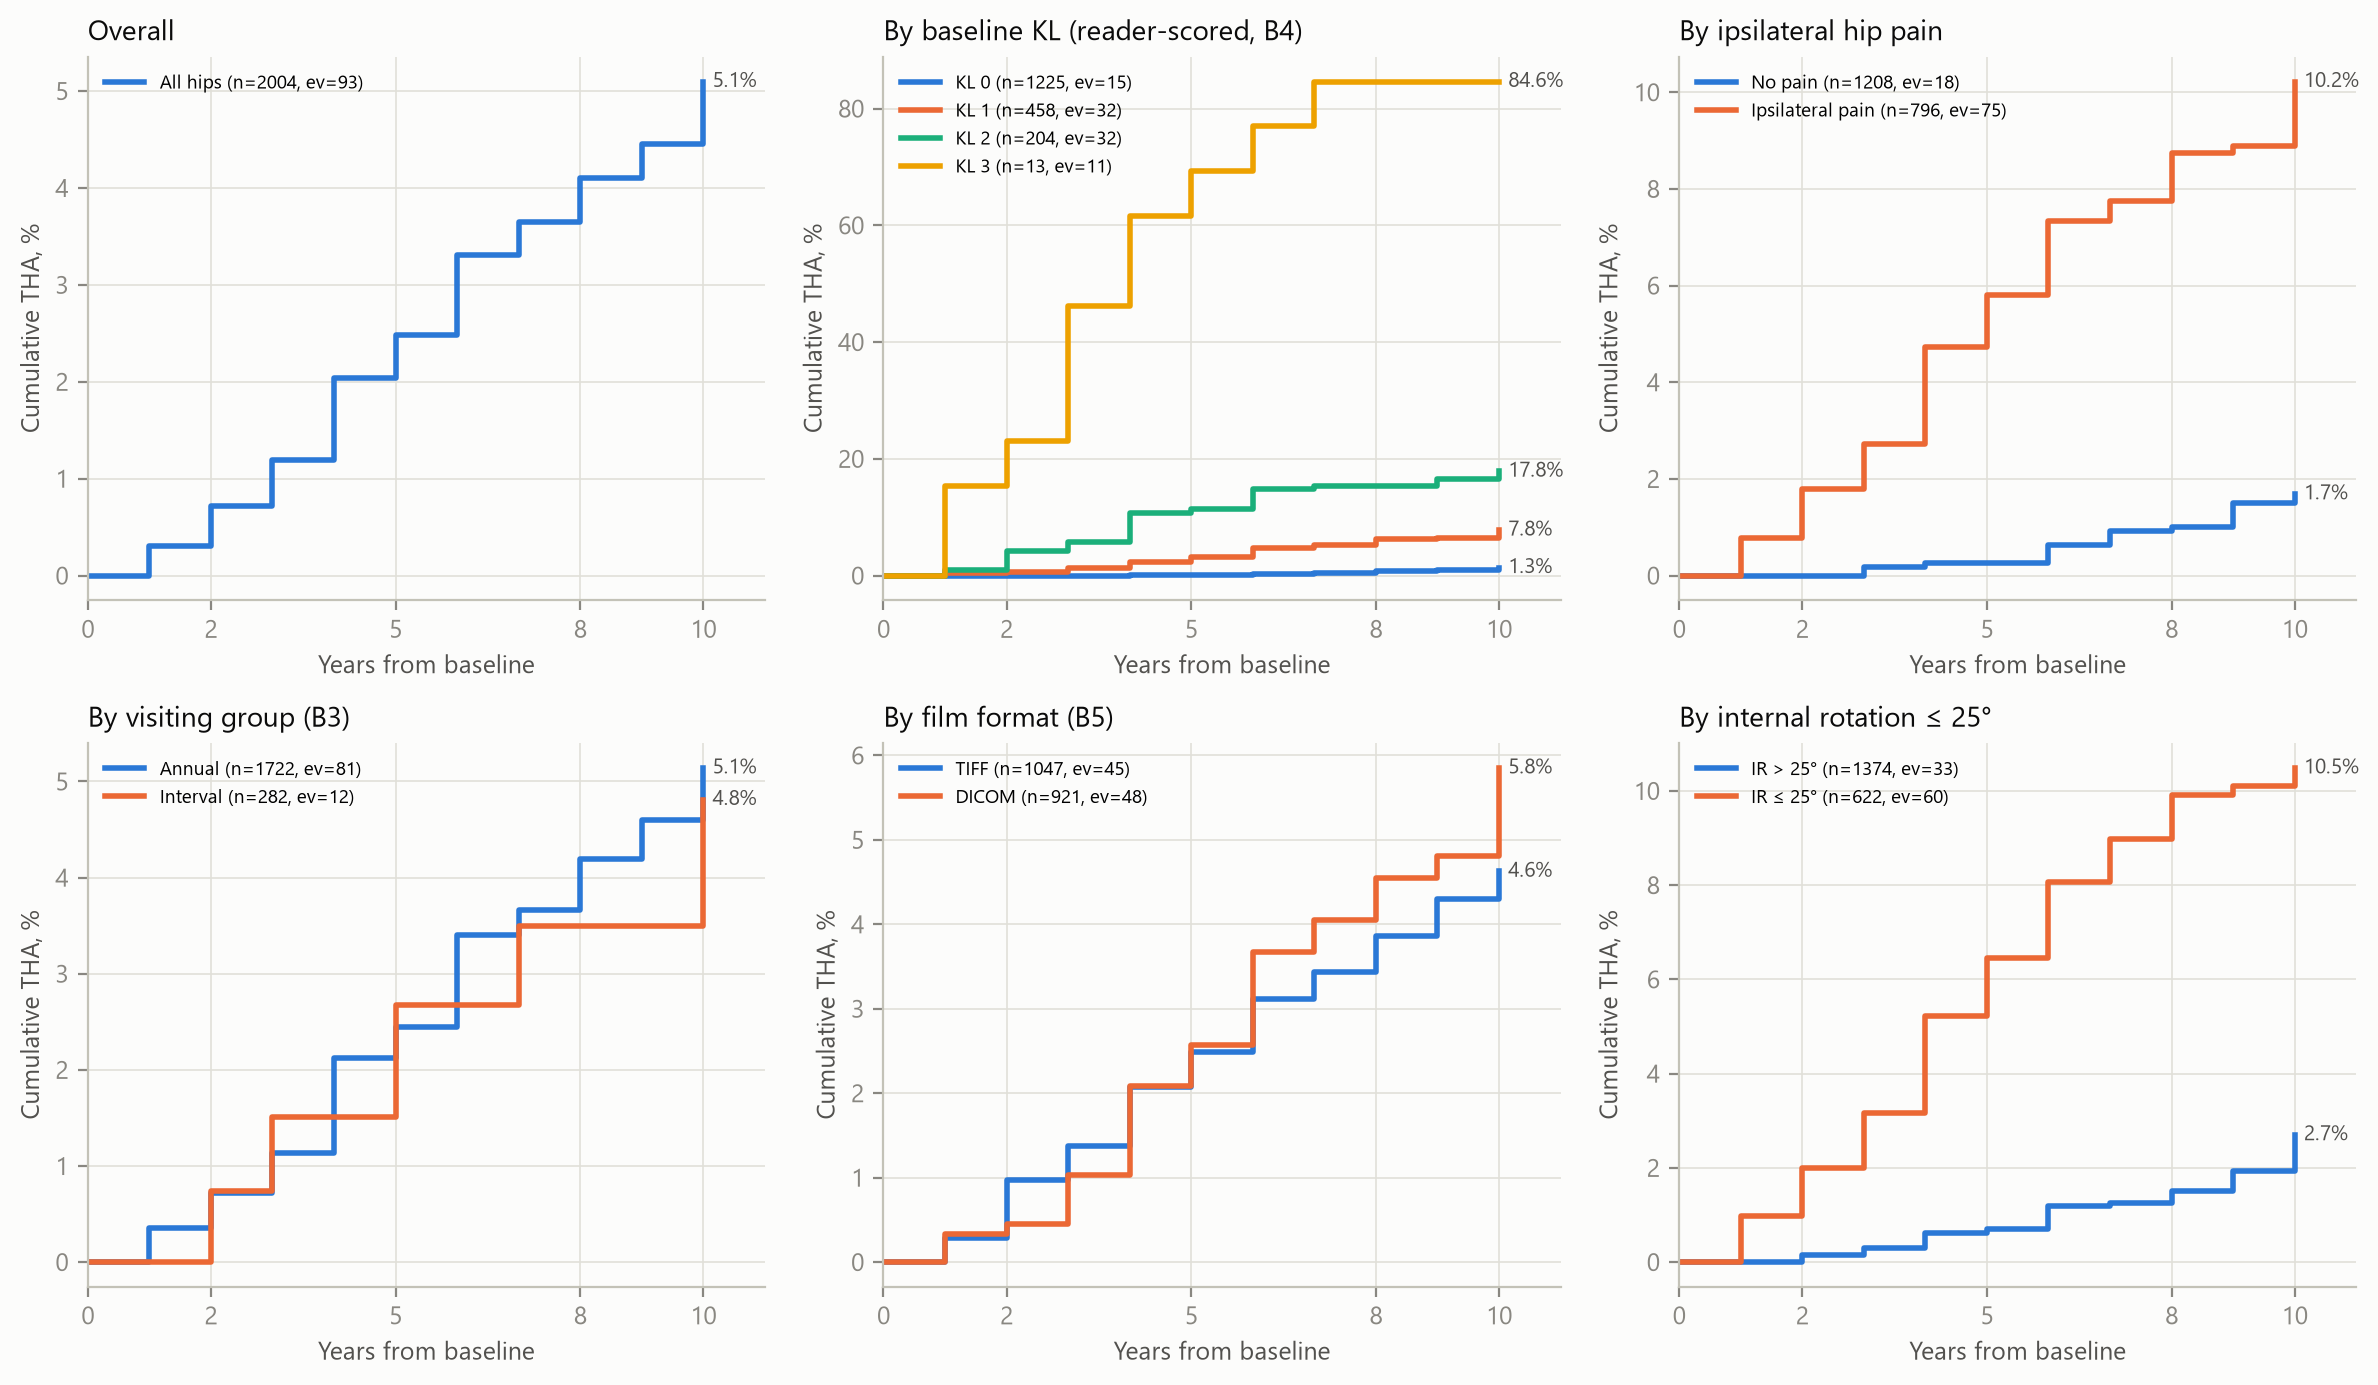
\includegraphics[width=\linewidth]{figS2_km_strata.png}
  \caption{\textbf{Cumulative incidence of THA (Kaplan--Meier) by baseline stratum.} Overall 10-year risk is 5.1\%.
  Ipsilateral hip pain (10.2\% vs 1.7\%) and internal rotation $\le25^\circ$ (10.5\% vs 2.7\%) separate risk
  strongly, whereas visiting group and film format do not. The reader-scored KL panel is shown for description only;
  these readings are not model inputs (Fig.~\ref{fig:timeline}).}
  \label{fig:s-km}
\end{figure}

\begin{figure}[!htbp]
  \centering
  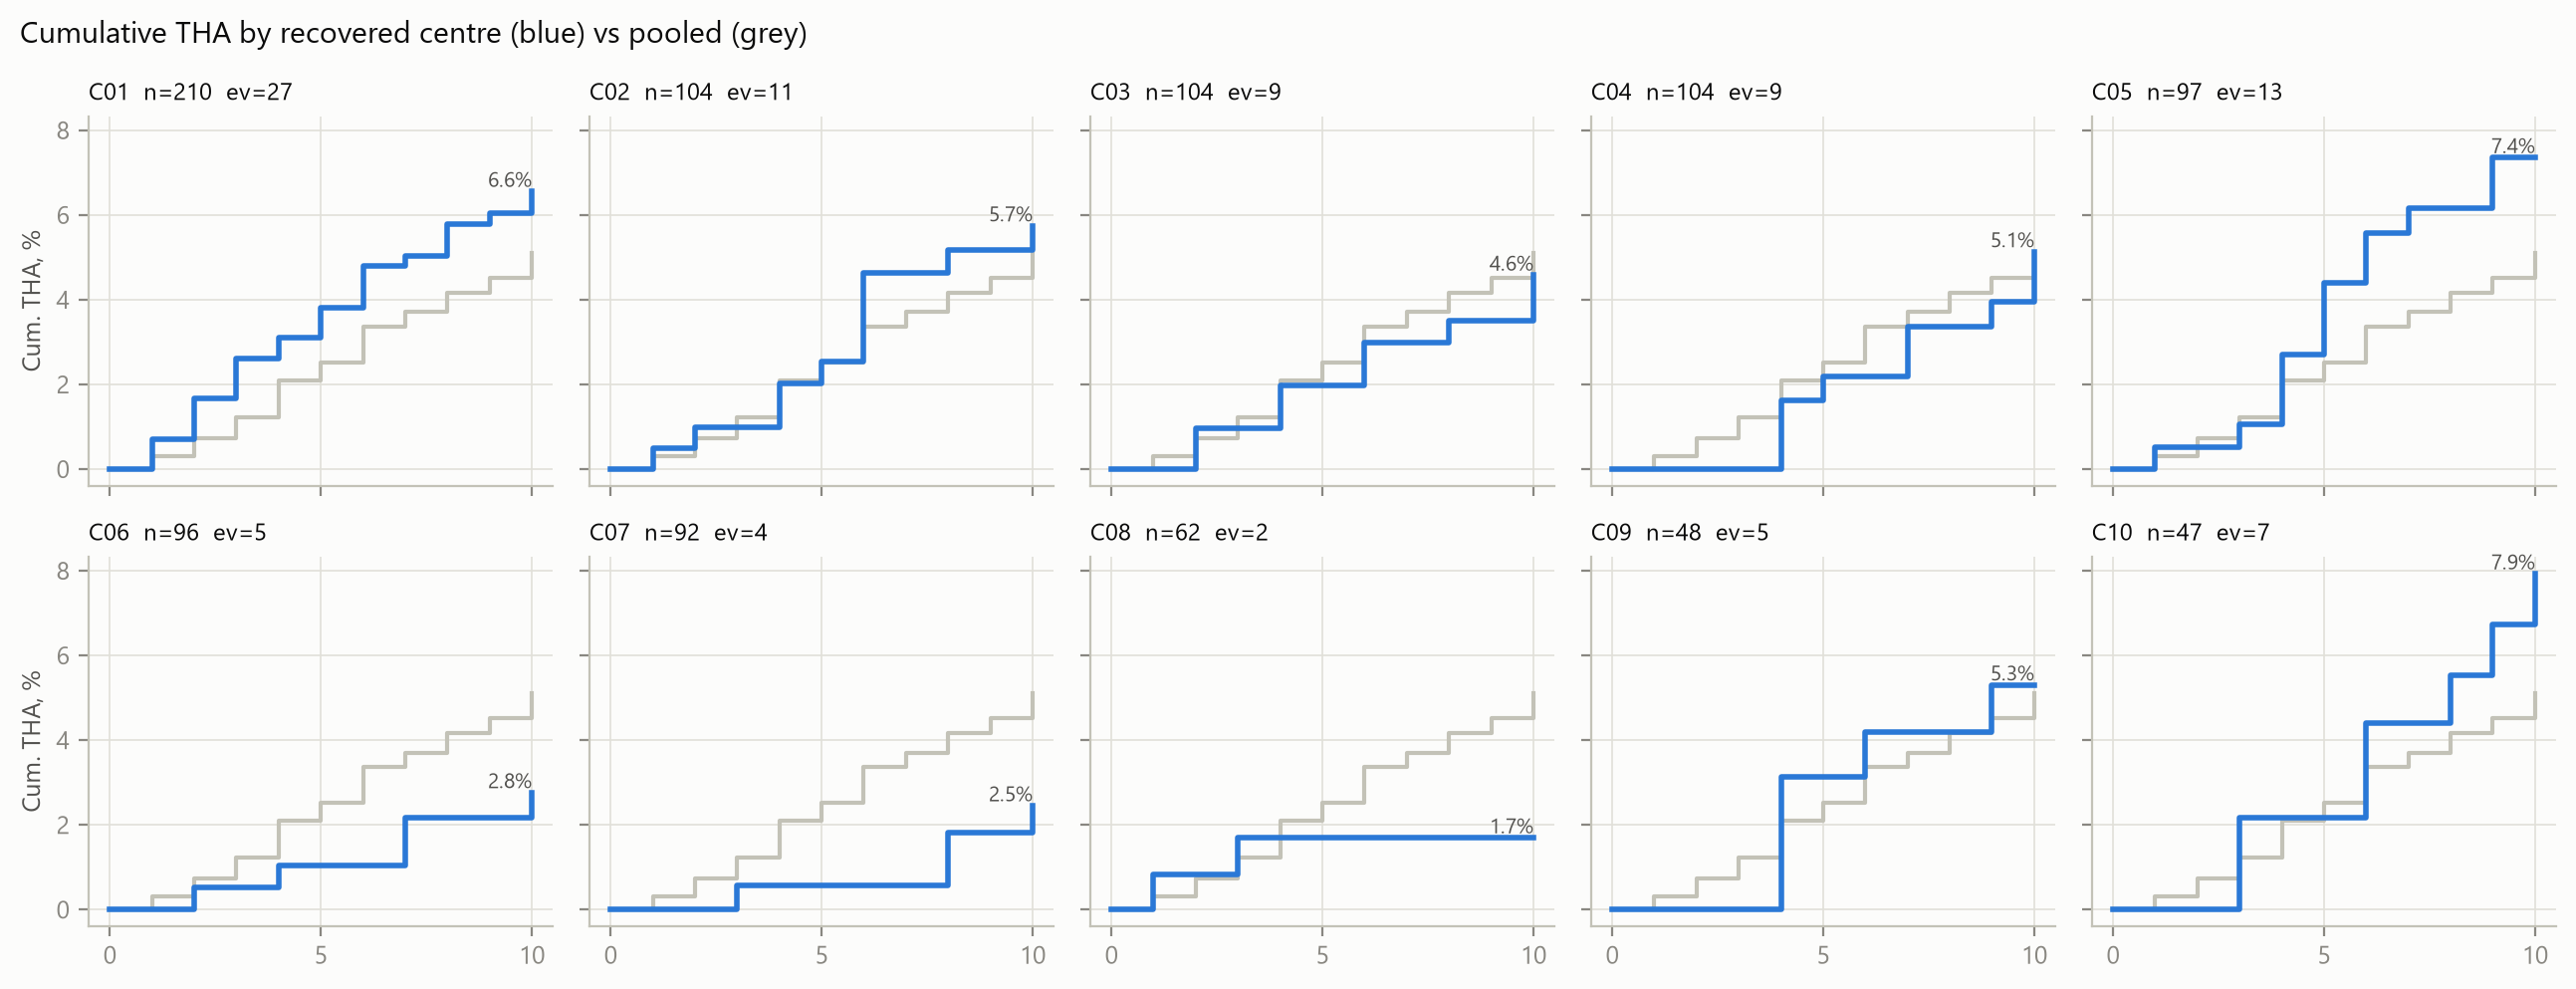
\includegraphics[width=\linewidth]{figS3_km_centre.png}
  \caption{\textbf{Cumulative incidence of THA by recovered centre} (blue) against the pooled curve (grey). Ten-year
  risk ranges from 1.7\% (C08, 2 events) to 7.9\% (C10, 7 events); the centre--outcome association is not significant
  (participant-clustered GEE $p=0.36$). Centre is metadata only, never a model input; it defines the
  leave-one-centre-out transport split.}
  \label{fig:s-km-centre}
\end{figure}

\begin{figure}[!htbp]
  \centering
  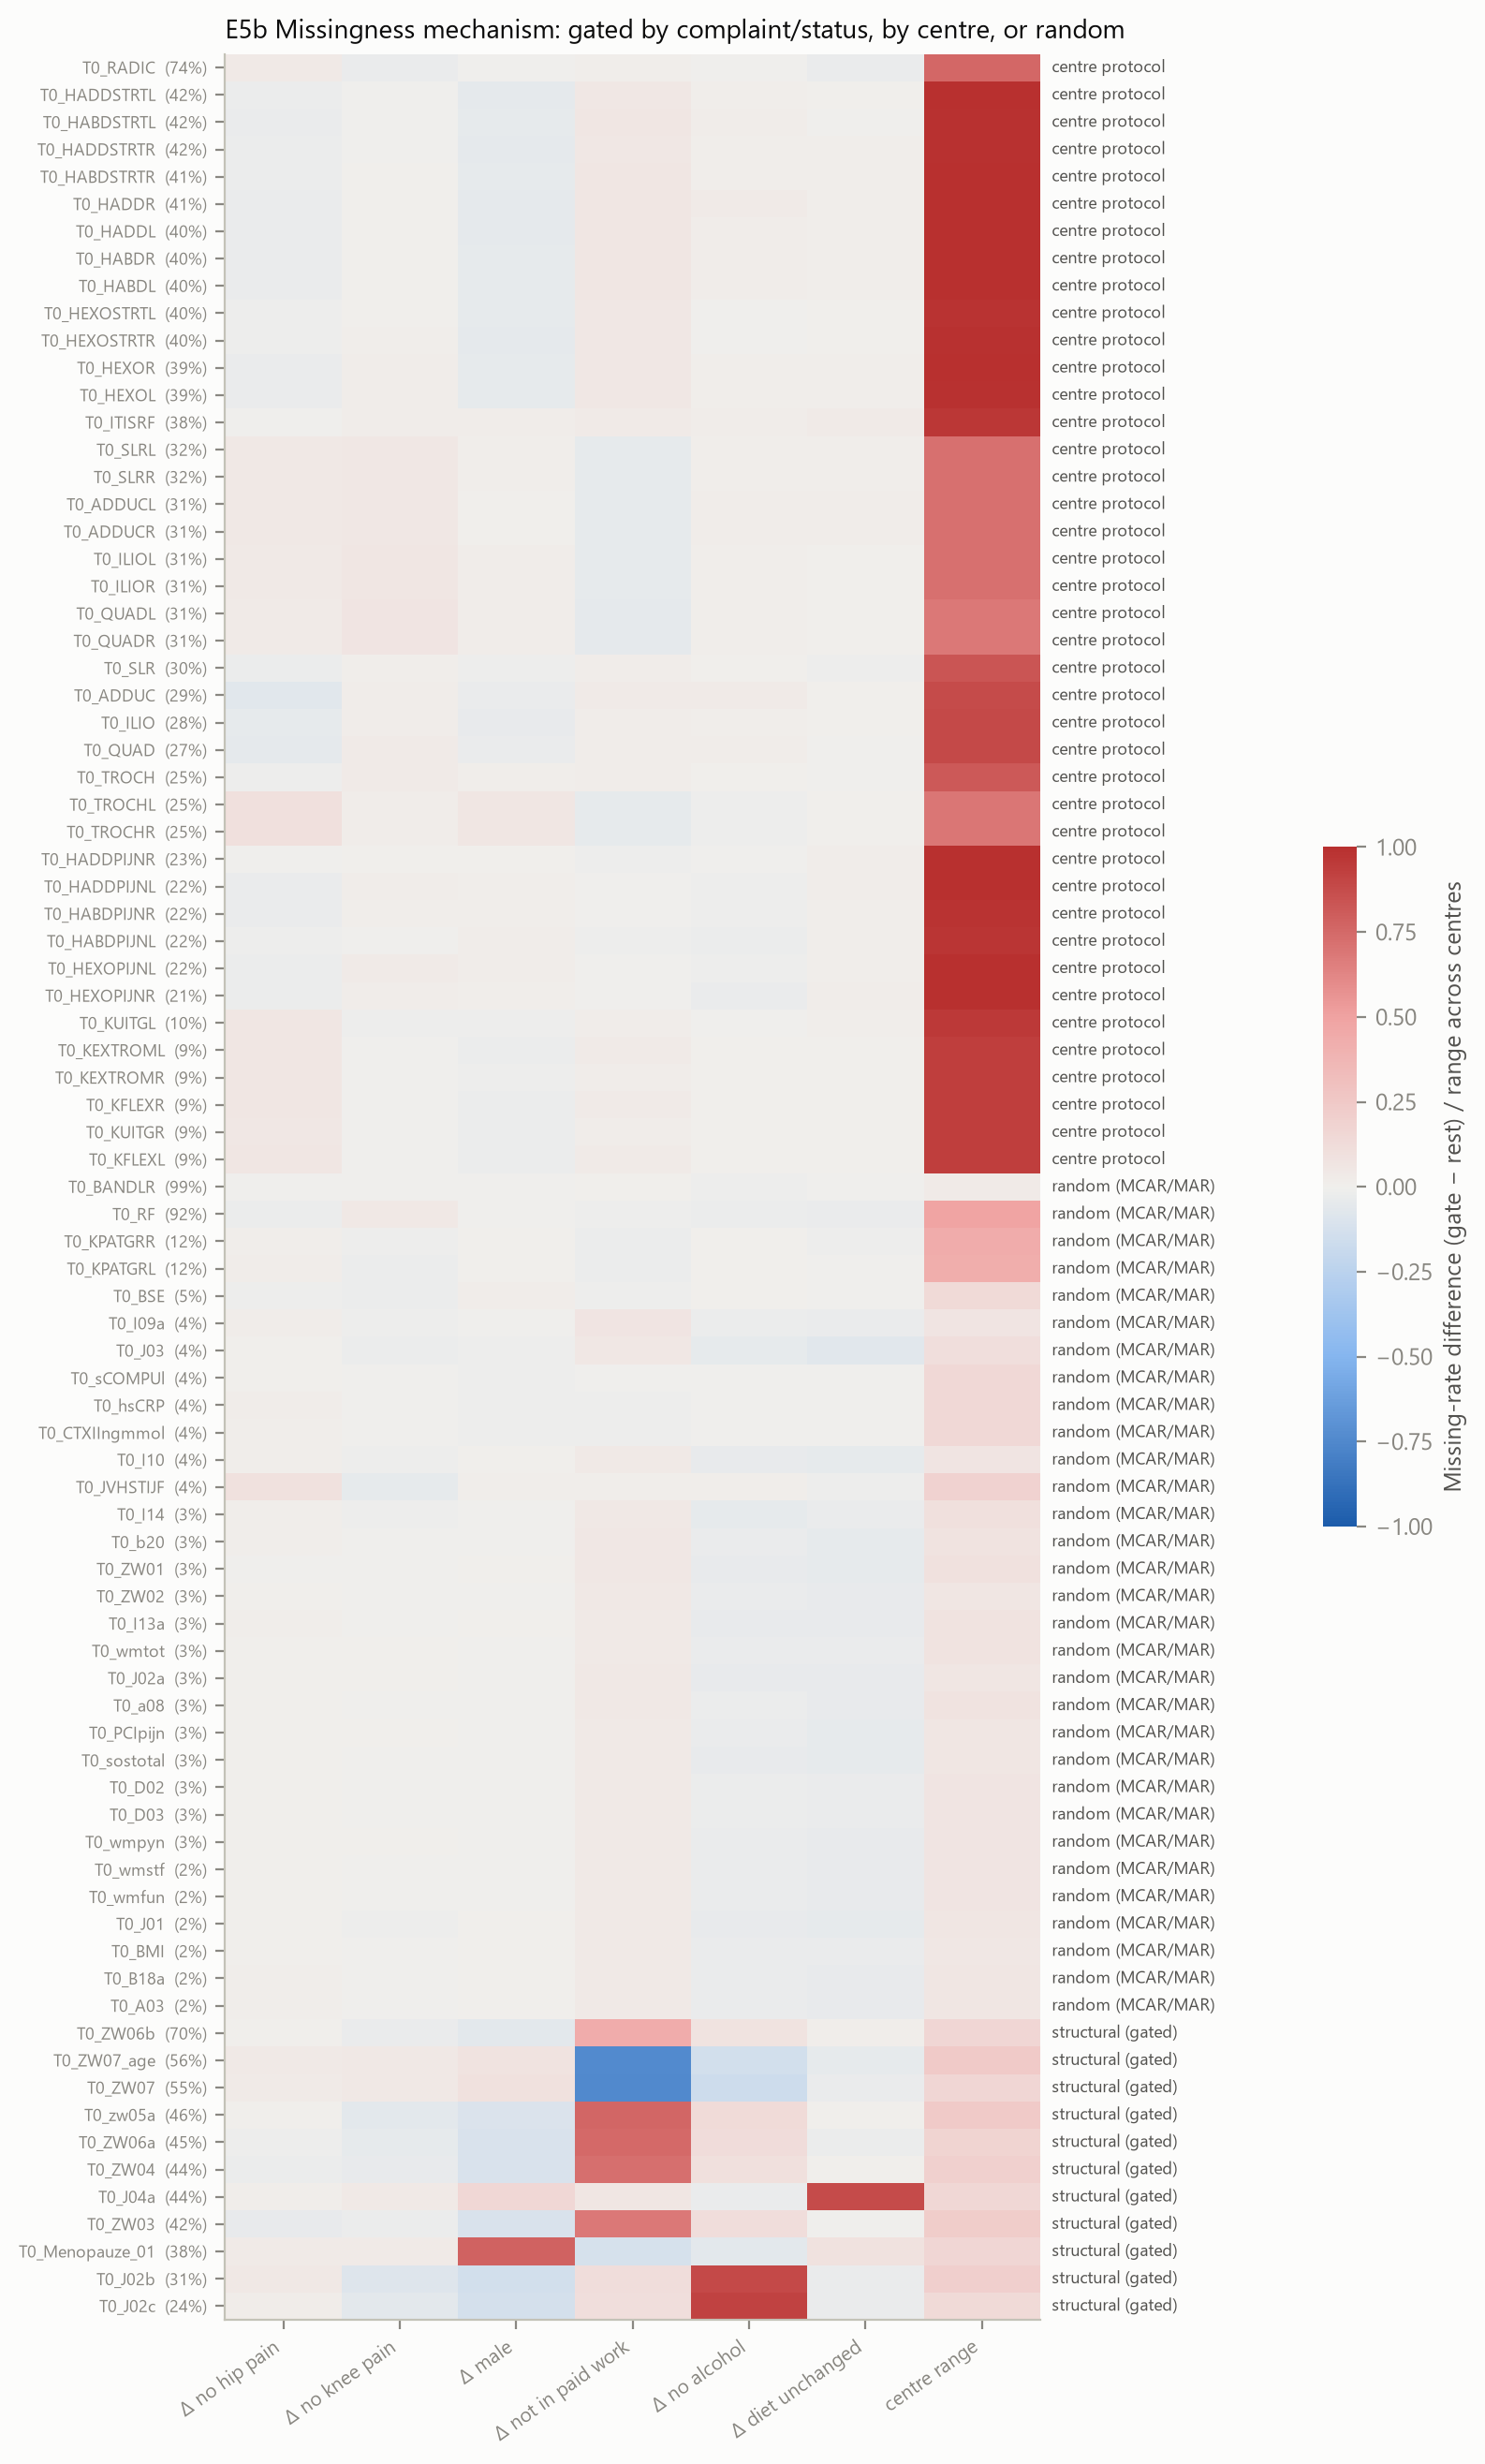
\includegraphics[width=0.82\linewidth]{figS4_missing_mechanism.png}
  \caption{\textbf{Missingness mechanism of every raw variable with $>$2\% missing.} Columns compare the missing rate
  between a gate (no hip pain, no knee pain, male, not in paid work, no alcohol, diet unchanged) and the rest, and give
  the range of missing rates across centres. Variables are classed as centre protocol (41; range near 1, e.g.\ external
  rotation, adduction and abduction ROM), structural / gated (38; coded by questionnaire logic) or sporadic (92; imputed
  fold-wise by MICE with indicators). Section~\ref{sec:methods} gives the rules.}
  \label{fig:s-missing}
\end{figure}

\begin{figure}[!htbp]
  \centering
  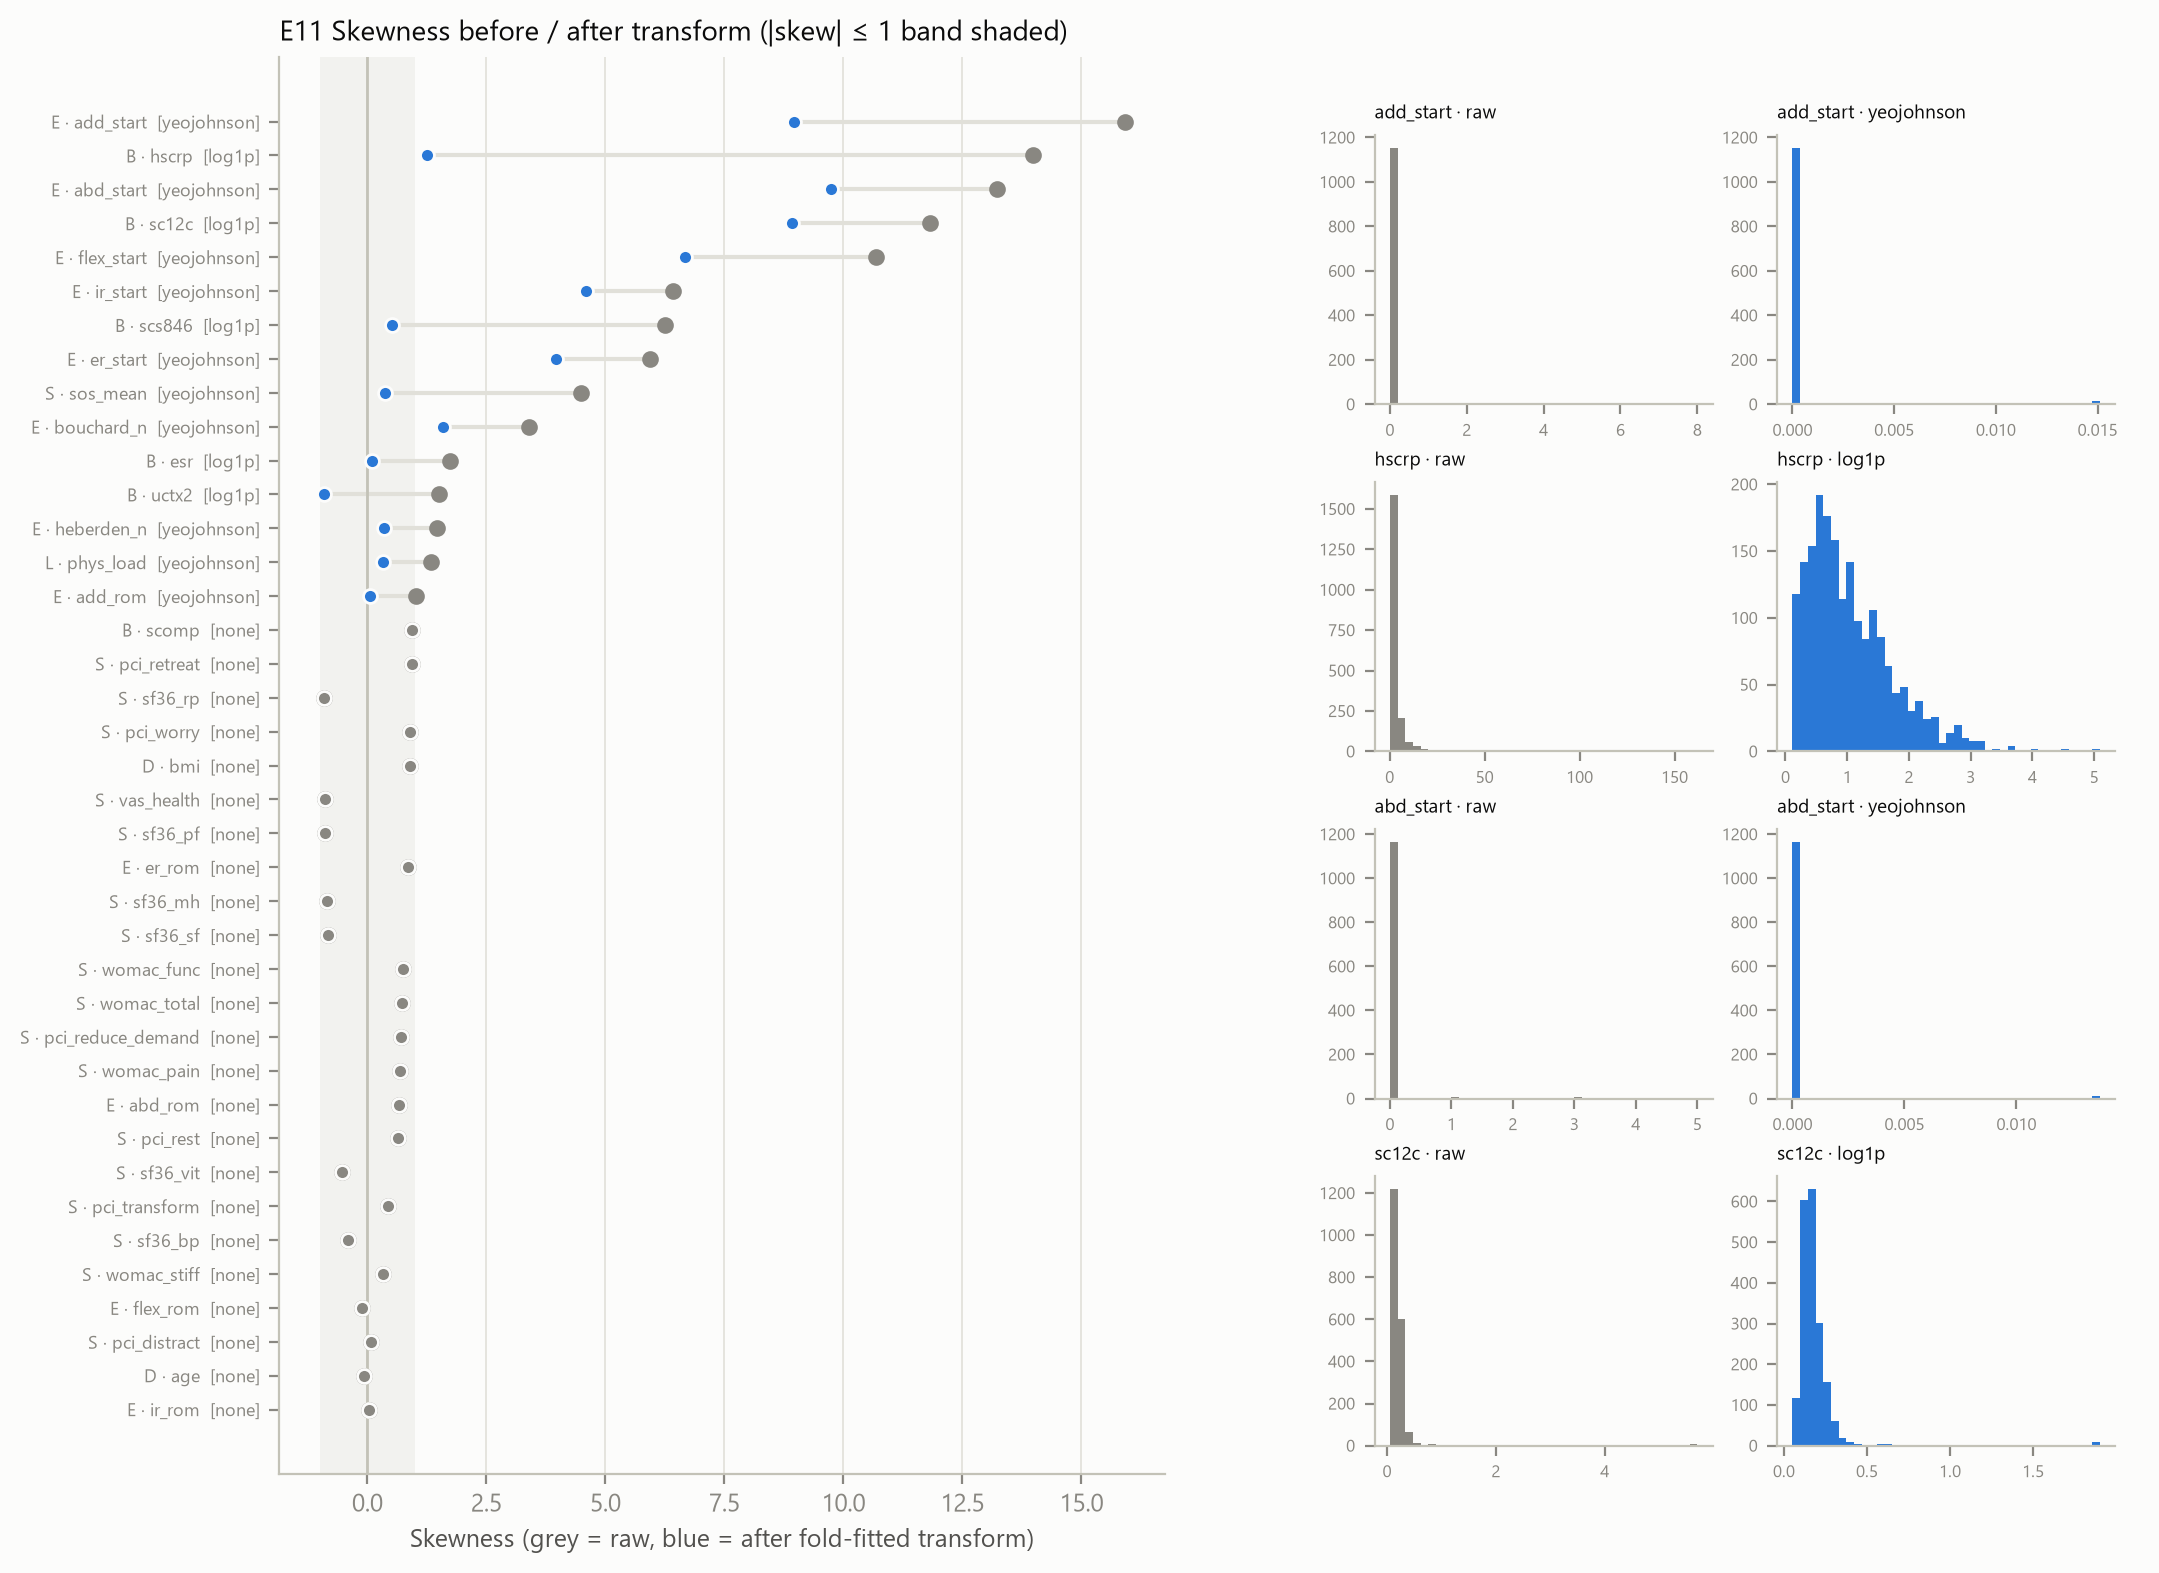
\includegraphics[width=\linewidth]{figS5_skewness.png}
  \caption{\textbf{Skewness before and after the fold-fitted transforms.} Fifteen continuous variables had
  $|\text{skew}|>1$. Biomarkers receive log1p (e.g.\ hsCRP 14 $\to$ 1.2) and other variables Yeo--Johnson, with
  $\lambda$ fitted on training rows, followed by winsorising at the training 0.5/99.5\% quantiles. Variables still
  skewed after transformation are zero-inflated goniometer start positions, which are not in the main set. Right:
  examples of raw and transformed distributions.}
  \label{fig:s-skew}
\end{figure}

\FloatBarrier
\setcounter{figure}{0}
\renewcommand{\thefigure}{A\arabic{figure}}

\section{Pseudo-external transport (full table)}
\label{app:transport}

\begin{table}[!htbp]
  \centering
  \caption{\textbf{Transport of M0 (all clinical features).} The model is trained on source participants, with
  participants who have a hip in the target removed from the source. Platt calibration and the 80\%-sensitivity
  threshold are fitted in the source, and the model is applied unchanged to the target. ``Internal'' is the nested-CV
  out-of-fold performance on the same target hips. $\Delta$ is the paired participant bootstrap (500 draws).}
  \small
  \setlength{\tabcolsep}{3pt}
  \resizebox{\linewidth}{!}{%
  \begin{tabular}{@{}lccccccc@{}}
    \toprule
    Source $\to$ target & Events & AUPRC ext./int. & $\Delta$AUPRC (95\% CI) & AUROC ext./int. & Cal.\ int. & Cal.\ slope & Sens./spec. \\
    \midrule
    Leave-one-centre-out (pooled) & 92 & 0.374 / 0.377 & $-0.003$ ($-0.049$, 0.039) & 0.803 / 0.820 & $-0.10$ & 0.82 & 0.71 / 0.68 \\
    TIFF $\to$ DICOM & 48 & 0.353 / 0.375 & $-0.022$ ($-0.097$, 0.057) & 0.778 / 0.802 & 0.06 & 0.76 & 0.65 / 0.71 \\
    DICOM $\to$ TIFF & 45 & 0.421 / 0.413 & 0.008 ($-0.085$, 0.087) & 0.850 / 0.843 & $-0.41$ & 1.08 & 0.87 / 0.63 \\
    Annual $\to$ interval group & 12 & 0.211 / 0.172 & 0.039 ($-0.019$, 0.157) & 0.799 / 0.788 & 0.30 & 0.74 & 0.75 / 0.67 \\
    Painful $\to$ painless hips & 18 & 0.099 / 0.101 & $-0.001$ ($-0.136$, 0.064) & 0.673 / 0.679 & $-1.47$ & 1.00 & 0.72 / 0.52 \\
    Female $\to$ male & 25 & 0.594 / 0.565 & 0.029 ($-0.060$, 0.100) & 0.903 / 0.902 & 0.28 & 1.39 & 0.92 / 0.62 \\
    High $\to$ low education & 65 & 0.406 / 0.420 & $-0.014$ ($-0.070$, 0.053) & 0.797 / 0.817 & 0.05 & 0.89 & 0.78 / 0.60 \\
    Low $\to$ high education & 26 & 0.318 / 0.365 & $-0.047$ ($-0.188$, 0.084) & 0.810 / 0.823 & $-0.41$ & 0.83 & 0.77 / 0.66 \\
    Prior care $\to$ none & 40 & 0.287 / 0.306 & $-0.018$ ($-0.082$, 0.061) & 0.806 / 0.789 & $-0.47$ & 0.71 & 0.70 / 0.74 \\
    No prior care $\to$ care & 52 & 0.354 / 0.481 & $\mathbf{-0.128}$ ($-0.220$, $-0.028$) & 0.807 / 0.848 & 0.08 & 1.22 & 0.94 / 0.40 \\
    \bottomrule
  \end{tabular}}
\end{table}

Per-centre calibration intercepts ranged from $-1.64$ (C08, 2 events) to $+1.37$ (C10, 7 events).
Image head (residual + OARSI; one fit per split, no bootstrap; internal reference = repeat-0 out-of-fold scores):
leave-one-centre-out AUROC/AUPRC 0.858/0.483 (internal 0.876/0.526); TIFF$\to$DICOM 0.813/0.465 (0.872/0.583);
DICOM$\to$TIFF 0.844/0.369 (0.883/0.495).

\section{Leakage audit of the code}
\label{app:audit}
Every fitted transformation, selection and calibration step was traced to the rows it was fitted on. Three deviations
from strict nesting were found, none of which touches M0 or the final fusion model.
\begin{enumerate}[itemsep=0pt]
  \item NAS stage 1 scored architectures on one outer split (repeat 0, fold 0), which is a test fold in 24 other splits.
        This affects M2 and M4.
  \item The SimCLR checkpoint was selected by a linear probe on the labels of the same split. This affects only the
        SimCLR variants.
  \item The pain and format domains of the transport experiment were first defined per hip, which placed 329
        participants on both sides of the split. This is \textbf{fixed}: the table above uses participant-disjoint
        sources.
\end{enumerate}
Label-free global steps are disclosed in Section~\ref{sec:methods}. The inner selection of the fusion model uses
singly, not doubly, cross-fitted logits; this is a second-order effect on tuning only.

\section{Links to the course lectures}
\label{app:lectures}
Slides refer to the MD6329 lecture PDFs; times refer to the lecture recordings
(\url{https://www.youtube.com/playlist?list=PLORG7zBQosxw}). We list only the points where this study uses or departs
from a technique covered in the course.

\begin{table}[!htbp]
  \centering
  \small
  \setlength{\tabcolsep}{4pt}
  \begin{tabular}{@{}p{0.43\linewidth}p{0.2\linewidth}p{0.13\linewidth}p{0.17\linewidth}@{}}
    \toprule
    Point in this report & Slides & Recording & Section \\
    \midrule
    Frozen ImageNet features as a feature extractor (our first image baseline; Bar et al.) & L02 p.\,102, 126--127 & 1:00--1:05 & Methods M3; Results \\
    How much data deep learning needs; transfer learning, which layers to freeze & L02 p.\,106--114 & 0:54--0:56 & Methods M3; Limitation 1 \\
    DenseNet-121 on radiographs (CheXNet) and saliency maps & L02 p.\,158; L11 p.\,34--35 & 1:29--1:31 & Methods M3; Fig.~\ref{fig:attention} \\
    Precision--recall for imbalanced data (AUPRC as primary metric) & L02 p.\,95 & -- & Results \\
    Class-weighted loss for imbalance (inverse class frequency; our pos\_weight) & L03 p.\,63--64 & 0:31--0:34 & Methods \\
    Dice and Jaccard overlap (our locator evaluation) & L03 p.\,65 & -- & Results \\
    Early / joint / late fusion (our token, FiLM and logit fusion) & L08 p.\,30 & 0:11--0:14 & Methods; Discussion \\
    Self-supervised learning, SimCLR & L08 p.\,42--50 & 0:17--0:20 & Methods; Results \\
    Attention as interpretability & L11 p.\,5 & -- & Results \\
    Occlusion, saliency, CAM (our attention maps) & L11 p.\,15--33 & 0:15--0:24 & Results \\
    Is model confidence trustworthy? (calibration) & L11 p.\,40 & 0:28--0:33 & Results \\
    Performance differences across populations (transport splits) & L11 p.\,45 & 0:28--0:33 & Results \\
    \bottomrule
  \end{tabular}
\end{table}

\section{Software 3.0 statement}
An AI coding agent (Claude Opus 5.5, used through Claude Code) took part in problem formulation, coding and evaluation.
Every suggestion was checked against the data, the code or the source paper before it was used, and several were rejected
or changed (below).

\paragraph{What the AI did.}
\begin{itemize}[leftmargin=*,itemsep=1pt]
  \item \emph{Problem formulation and literature.} It ran scripted searches of the Europe PMC API (six query families, 208
        unique records, 49 abstracts read in full) and tabulated cohorts, endpoints and metrics (Table~\ref{tab:forest}).
        It also wrote the feasibility analysis: data access per candidate dataset, the size of the imaging work, and
        benchmark-based estimates of training time for each model on a CPU-only laptop.
  \item \emph{Image data curation.} It found that about 110 films were stored rotated by $90^\circ$ and built the
        self-supervised rotation fix. It also redesigned the femoral-head locator's decoding, which cut gross errors from
        19\% to 1.8\%.
  \item \emph{Model engineering and audit.} It wrote most of the pipeline code. It found that the discrete-time head
        never trained (zero-initialised hazard bias). It traced M2's instability to early stopping on about 25 noisy
        validation events, using the per-repeat SD and the distribution of stopping epochs. It audited the code line by
        line for train/test leakage (Appendix~\ref{app:audit}), which led to the participant-disjoint transport splits.
  \item \emph{Interpretation and writing support.} It drafted the interpretation of part of the experimental results,
        produced the data-driven figures, and proofread the report.
\end{itemize}

\paragraph{What the author did.}
\begin{itemize}[leftmargin=*,itemsep=1pt]
  \item \emph{Topic and question.} Chose CHECK after weighing dataset accessibility. Defined the clinical problem: 10-year ipsilateral THA as the endpoint instead of radiographic OA, rare
        events treated as a feature of the problem, and first presentation as the prediction time.
  \item \emph{Features and design.} Selected the feature groups and the redundancy and missingness rules. Designed the
        experiments: nested repeated grouped CV instead of a 20\% hold-out, no SMOTE, leave-one-centre-out as the main
        transport split, and no language model.
  \item \emph{Architecture.} Chose and optimised the architectures: SimCLR with forgetting guards, the dual-head
        FT-Transformer, and the decision to supervise the image branch after its first version underperformed.
  \item \emph{Validity checks.} Rejected label permutation and KL stratification as sufficient evidence against leakage
        and required the temporal audit, which defined the admissibility of every input at $t_0$.
  \item \emph{Analysis and writing.} Designed the auxiliary analyses and analysed their results. Wrote the narrative
        logic and most of the content of this report.
\end{itemize}

\paragraph{Effect on the workflow.} The agent made exhaustive checks cheap: line-by-line leakage tracing, rerunning all
five repeats, verifying literature numbers against full texts. It also exposed errors that a single pass would have
missed, such as the rotated films, the untrained head and the hip-level transport split. Its own suggestions also needed
correcting. It initially proposed using the OARSI items as auxiliary targets, then withdrew the idea as leakage-prone; it
was later reinstated as targets only, after the temporal audit. Every number in the report was regenerated from saved
out-of-fold predictions by scripts in the supplementary material and the code repository (\url{\repourl}).
